%
%===================================================================================================
%
\documentclass[aspectratio=169, 11pt]{beamer}

%
%===================================================================================================
%
% Theme & Colors 

\usetheme{Madrid}
\usecolortheme{whale}

\definecolor{darkblue}{RGB}{0,51,102}
\definecolor{lightgray}{RGB}{240,240,240}
\definecolor{accent}{RGB}{180,40,40}
\definecolor{darkgreen}{RGB}{0,100,60}

\setbeamercolor{frametitle}{bg=darkblue, fg=white}
\setbeamercolor{title}{bg=darkblue, fg=white}
\setbeamercolor{block title}{bg=darkblue, fg=white}
\setbeamercolor{block body}{bg=lightgray}
\setbeamercolor{block title alerted}{bg=accent, fg=white}
\setbeamercolor{block body alerted}{bg=red!5}
\setbeamercolor{block title example}{bg=darkgreen, fg=white}
\setbeamercolor{block body example}{bg=green!5}
\setbeamertemplate{navigation symbols}{}
\setbeamertemplate{footline}[frame number]

%
%===================================================================================================
%
% Packages 

\usepackage[utf8]{inputenc}
\usepackage[T1]{fontenc}
\usepackage{graphicx}
\usepackage{booktabs}
\usepackage{listings}
\usepackage{xcolor}
\usepackage{tikz}
\usetikzlibrary{arrows.meta, positioning, shapes.geometric, calc, fit, decorations.pathreplacing}
\usepackage{amsmath, amssymb}

%
%===================================================================================================
%
% Listings style 

\lstset{
  language=Python,
  basicstyle=\ttfamily\scriptsize,
  keywordstyle=\color{blue}\bfseries,
  stringstyle=\color{red!70!black},
  commentstyle=\color{green!50!black}\itshape,
  backgroundcolor=\color{lightgray},
  frame=single,
  framerule=0.4pt,
  rulecolor=\color{gray},
  breaklines=true,
  showstringspaces=false,
  columns=fullflexible,
  xleftmargin=4pt,
  xrightmargin=4pt,
  aboveskip=6pt,
  belowskip=4pt,
}

%
%===================================================================================================
%
% Title page information

\author{Giovanni Della Lunga\\{\footnotesize giovanni.dellalunga@unibo.it}}
\title{Chapter 4\\Learning and Evaluating Cross-Sectional Return Predictors}
\subtitle{Asset Pricing \& Machine Learning in Finance} % (optional)
\setbeamercovered{transparent} 
\institute{Advanced Topics in Artificial Intelligence} 
\date{Bologna - March, 2026} 
%
%===================================================================================================
%
\begin{document}
%
%===================================================================================================
%
\setbeamertemplate{subsection page}
{
  \begingroup
    %\begin{beamercolorbox}[sep=12pt,center]{section title}
      %\usebeamerfont{section title}
	  \centering 	     
      Section~\insertsectionnumber.\insertsubsectionnumber\par 
      \vspace{1cm}
    %\end{beamercolorbox}
    %\vspace*{-2pt}
    \begin{beamercolorbox}[sep=8pt,center,rounded=true]{title}
      \usebeamerfont{section title}
      \insertsubsection\par
    \end{beamercolorbox}
  \endgroup
}
%
%===================================================================================================
%
\AtBeginSection[]
{
  %\begin{frame}<beamer>
  %\footnotesize	
  %\frametitle{Outline}
  %\begin{multicols}{2}
  %\tableofcontents[currentsection]
  %\end{multicols}	  
  %\normalsize
  %\end{frame}
  \begin{frame}
  \vfill
  \centering
  \begin{beamercolorbox}[sep=8pt,center,shadow=true,rounded=true]{title}  	\usebeamerfont{title}\insertsectionhead\par%
  \end{beamercolorbox}
  \vfill
  \end{frame}
}
\AtBeginSubsection{\frame{\subsectionpage}}
%
%===================================================================================================
%
\begin{frame}
\titlepage
\end{frame}
%
%===================================================================================================
%
\begin{frame}{Contents}
%\begin{multicols}{2}
\tableofcontents[
    sectionstyle=show,
    subsectionstyle=show
]
%\end{multicols}
\end{frame}
%__________________________________________________________________________
%
\section{Model Architecture, Training \& Evaluation}
%__________________________________________________________________________
%
%
%..................................................................
%
\begin{frame}{Where We Are in the Project}

\begin{columns}[T]
\column{0.52\textwidth}
\begin{block}{Part~1 (Previous Chapter)}
\begin{itemize}
  \item Downloaded prices \& metadata
  \item Constructed weekly returns
  \item Engineered 15 firm-level characteristics
  \item Stored everything in HDF5
\end{itemize}
\end{block}

\begin{alertblock}{Part~2 (This Chapter)}
\begin{itemize}
  \item Load \& preprocess the dataset
  \item Build the conditional autoencoder in Keras
  \item Walk-forward cross-validation
  \item Hyperparameter search \& evaluation
  \item Generate out-of-sample predictions
\end{itemize}
\end{alertblock}

\column{0.44\textwidth}
\centering
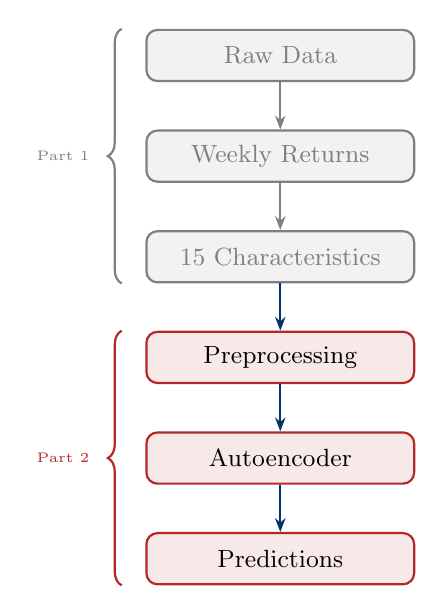
\begin{tikzpicture}[
  node distance=0.6cm,
  box/.style={draw=darkblue, thick, rounded corners, fill=darkblue!10,
              minimum width=3.4cm, minimum height=0.65cm, align=center, font=\small},
  done/.style={box, draw=gray, fill=gray!10, text=gray},
  curr/.style={box, draw=accent, fill=accent!10},
  arr/.style={-{Stealth[length=5pt]}, thick, darkblue}
]
\node[done] (d1) {Raw Data};
\node[done, below=of d1] (d2) {Weekly Returns};
\node[done, below=of d2] (d3) {15 Characteristics};
\node[curr, below=of d3] (d4) {Preprocessing};
\node[curr, below=of d4] (d5) {Autoencoder};
\node[curr, below=of d5] (d6) {Predictions};

\draw[arr, gray] (d1) -- (d2);
\draw[arr, gray] (d2) -- (d3);
\draw[arr] (d3) -- (d4);
\draw[arr] (d4) -- (d5);
\draw[arr] (d5) -- (d6);

\draw[decorate, decoration={brace, amplitude=5pt, mirror}, thick, gray]
  ([xshift=-0.3cm]d1.north west) -- ([xshift=-0.3cm]d3.south west)
  node[midway, left=8pt, font=\tiny, gray] {Part 1};
\draw[decorate, decoration={brace, amplitude=5pt, mirror}, thick, accent]
  ([xshift=-0.3cm]d4.north west) -- ([xshift=-0.3cm]d6.south west)
  node[midway, left=8pt, font=\tiny, accent] {Part 2};
\end{tikzpicture}
\end{columns}

\end{frame}
%__________________________________________________________________________
%
\subsection{The Conditional Autoencoder}
%__________________________________________________________________________
%
\begin{frame}[fragile]{Loading \& Merging Returns and Characteristics}

\begin{lstlisting}
# Load weekly returns from HDF5, reshape to long format, filter from 1993
data = (pd.read_hdf(results_path / 'autoencoder_reloaded.h5', 'returns')
        .stack(dropna=False).to_frame('returns')
        .loc[idx['1993':, :], :])

# Merge all 15 firm characteristics from HDF5
with pd.HDFStore(results_path / 'autoencoder_reloaded.h5') as store:
    keys = [k[1:] for k in store.keys() if k[1:].startswith('factor')]
    for key in keys:
        data[key.split('/')[-1]] = store[key].squeeze()
\end{lstlisting}
\end{frame}
%
%..................................................................
%
\begin{frame}[fragile]{Loading \& Merging Returns and Characteristics}

\begin{block}{Resulting Panel Structure}
\centering\small
\begin{tabular}{llccccc}
\toprule
\textbf{date} & \textbf{ticker} & \textbf{returns} & \textbf{beta} & \textbf{mom12m} & $\cdots$ & \textbf{retvol} \\
\midrule
1993-01-08 & AAPL & 0.012 & 1.23 & 0.15 & $\cdots$ & 0.032 \\
1993-01-08 & MSFT & 0.007 & 0.98 & 0.22 & $\cdots$ & 0.028 \\
$\vdots$ & $\vdots$ & $\vdots$ & $\vdots$ & $\vdots$ & & $\vdots$ \\
\bottomrule
\end{tabular}

\medskip
MultiIndex \texttt{(date, ticker)} $\times$ 16 columns (1 return + 15 characteristics)
\end{block}

\end{frame}
%
%..................................................................
%
\begin{frame}[fragile]{Forward Returns \& Rank Normalisation}

\begin{columns}[T]
\column{0.48\textwidth}
\begin{block}{Target Variable: $r_{i,t+1}$}
\begin{lstlisting}
data['returns_fwd'] = (
    data.returns
    .unstack('ticker')
    .shift(-1)   # align t+1 with t
    .stack())
\end{lstlisting}
The model predicts \textbf{next-week} returns using information available \textbf{today}.
\end{block}

\column{0.48\textwidth}
\begin{block}{Rank Normalisation}
\begin{lstlisting}
data.loc[:, characteristics] = (
  data[characteristics]
  .groupby(level='date')
  .apply(lambda x: pd.DataFrame(
    quantile_transform(x,
      n_quantiles=x.shape[0]),
    columns=characteristics,
    index=x.index.get_level_values(
      'ticker')))
  .mul(2).sub(1))
\end{lstlisting}
\end{block}
\end{columns}
\end{frame}
%
%..................................................................
%
\begin{frame}[fragile]{Forward Returns \& Rank Normalisation}

\begin{block}{Why Rank-Normalise?  (Kelly et al., 2019)}
\begin{itemize}
  \item Cross-sectional \texttt{quantile\_transform} maps each characteristic to $[0,1]$, then rescaled to $(-1,+1)$
  \item Removes outliers, makes features comparable in scale across dates
  \item Preserves the \textbf{ranking} of stocks --- the model only needs ordinal information
\end{itemize}
\end{block}

\end{frame}
%
%..................................................................
%
\begin{frame}[fragile]{Final Preprocessing Steps}

Three additional cleaning operations before model training:

\vspace{0.3cm}

\begin{columns}[T]
\column{0.32\textwidth}
\begin{block}{Date Filter}
\begin{lstlisting}
data = data.loc[
    idx[:'2019', :], :]
\end{lstlisting}
Restrict to data ending in 2019 for a clean backtesting period.
\end{block}

\column{0.32\textwidth}
\begin{block}{Return Clipping}
\begin{lstlisting}
data.loc[:,
  ['returns','returns_fwd']] = \
  data.loc[:,
  ['returns','returns_fwd']] \
  .clip(lower=-1, upper=1.0)
\end{lstlisting}
Cap extreme returns at $\pm100\%$ to limit the influence of outliers on MSE loss.
\end{block}

\column{0.32\textwidth}
\begin{block}{Missing Value Sentinel}
\begin{lstlisting}
data = data.fillna(-2)
\end{lstlisting}
Replace NaN with $-2$ (outside the $[-1,+1]$ range of normalised characteristics). This sentinel is filtered out when computing IC.
\end{block}
\end{columns}

\vspace{0.4cm}

The processed dataset is saved to HDF5 under key \texttt{model\_data} for reproducibility.

\end{frame}
%
%..................................................................
%
\begin{frame}{Conditional Autoencoder --- Conceptual View}

\centering
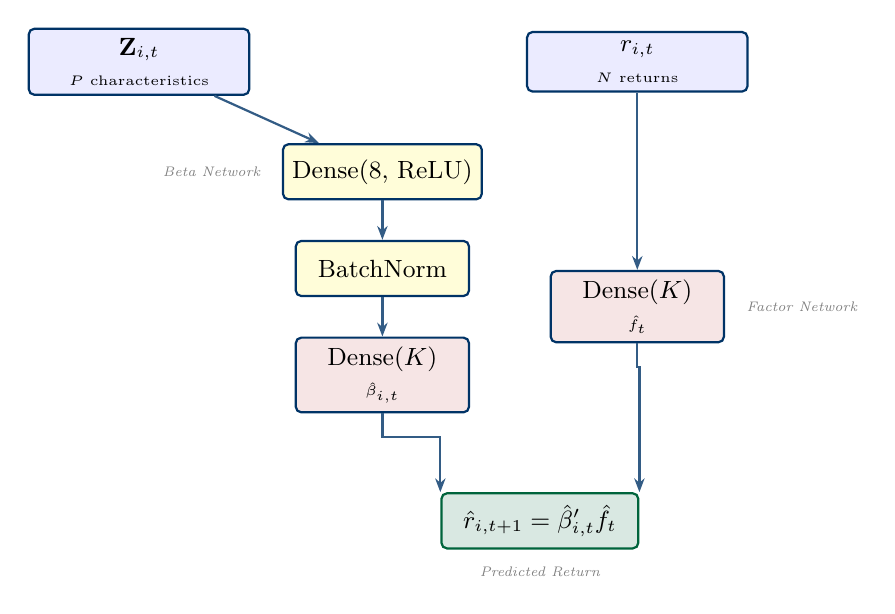
\begin{tikzpicture}[
  node distance=0.5cm and 1.0cm,
  layer/.style={draw=darkblue, thick, rounded corners=2pt, minimum height=0.7cm,
                align=center, font=\small},
  input/.style={layer, fill=blue!8, minimum width=2.8cm},
  hidden/.style={layer, fill=yellow!15, minimum width=2.2cm},
  output/.style={layer, fill=accent!12, minimum width=2.2cm},
  final/.style={layer, fill=darkgreen!15, minimum width=2.5cm, draw=darkgreen},
  arr/.style={-{Stealth[length=5pt]}, thick, darkblue!80},
  lbl/.style={font=\tiny\itshape, text=gray}
]

% Beta network (left branch)
\node[input] (ib) {$\mathbf{Z}_{i,t}$\\{\tiny $P$ characteristics}};
\node[hidden, below right=0.6cm and 0.4cm of ib] (h1) {Dense(8, ReLU)};
\node[hidden, below=0.5cm of h1] (bn) {BatchNorm};
\node[output, below=0.5cm of bn] (ob) {Dense($K$)\\{\tiny $\hat\beta_{i,t}$}};

% Factor network (right branch)
\node[input, right=3.5cm of ib] (ir) {$r_{i,t}$\\{\tiny $N$ returns}};
\node[output, below=2.25cm of ir] (of) {Dense($K$)\\{\tiny $\hat f_t$}};

% Dot product
\node[final, below=1.0cm of ob, xshift=2.0cm] (dot) {$\hat r_{i,t+1} = \hat\beta_{i,t}' \hat f_t$};

% Arrows
\draw[arr] (ib) -- (h1);
\draw[arr] (h1) -- (bn);
\draw[arr] (bn) -- (ob);
\draw[arr] (ir) -- (of);
\draw[arr] (ob.south) -- ++(0,-0.3) -| (dot.north west);
\draw[arr] (of.south) -- ++(0,-0.3) -| (dot.north east);

% Labels
\node[lbl, left=0.15cm of h1] {Beta Network};
\node[lbl, right=0.15cm of of] {Factor Network};
\node[lbl, below=0.1cm of dot] {Predicted Return};

\end{tikzpicture}

\vspace{0.2cm}

\begin{columns}[T]
\column{0.48\textwidth}
\begin{block}{Beta Network (Encoder)}
Maps $P=15$ firm characteristics $\mathbf{Z}_{i,t}$ to $K$ \textbf{conditional factor loadings} $\hat\beta_{i,t} \in \mathbb{R}^K$.
\end{block}

\column{0.48\textwidth}
\begin{block}{Factor Network (Decoder)}
Maps $N$ cross-sectional returns $r_{i,t}$ to $K$ \textbf{latent factors} $\hat f_t \in \mathbb{R}^K$.
\end{block}
\end{columns}

\end{frame}
%
%..................................................................
%
\begin{frame}[fragile]{Model in Keras Code}

\begin{lstlisting}
def make_model(hidden_units=8, n_factors=3):
    # --- Inputs ---
    input_beta   = Input((n_tickers, n_characteristics), name='input_beta')
    input_factor = Input((n_tickers,),                   name='input_factor')

    # --- Beta Network: characteristics -> factor loadings ---
    hidden_layer = Dense(hidden_units, activation='relu', name='hidden_layer')(input_beta)
    batch_norm   = BatchNormalization(name='batch_norm')(hidden_layer)
    output_beta  = Dense(n_factors, name='output_beta')(batch_norm)

    # --- Factor Network: returns -> latent factors ---
    output_factor = Dense(n_factors, name='output_factor')(input_factor)

    # --- Output: dot product beta' * f ---
    output = Dot(axes=(2,1), name='output_layer')([output_beta, output_factor])

    model = Model(inputs=[input_beta, input_factor], outputs=output)
    model.compile(loss='mse', optimizer='adam')
    return model
\end{lstlisting}

\vspace{0.2cm}
\end{frame}
%
%..................................................................
%
\begin{frame}[fragile]{Model in Keras Code}
\vspace{1cm}
Loss function: $\displaystyle\mathcal{L} = \frac{1}{NT}\sum_{i,t}\bigl(r_{i,t+1} - \hat\beta_{i,t}'\,\hat f_t\bigr)^2$\quad (MSE), optimised with \textbf{Adam}.

\end{frame}
%
%..................................................................
%
\begin{frame}{Understanding the Architecture}
\small
\begin{columns}[T]
\column{0.48\textwidth}
\begin{block}{Input Shapes}
\begin{itemize}
  \item \texttt{input\_beta}: $(T \times N \times P)$\\
        $T$ weeks, $N$ tickers, $P{=}15$ characteristics
  \item \texttt{input\_factor}: $(T \times N)$\\
        Contemporaneous returns matrix
\end{itemize}
\end{block}

\begin{block}{Key Design Choices}
\begin{itemize}
  \item \textbf{No activation} on output layers --- betas and factors are unconstrained linear projections
  \item \textbf{Dot product} enforces the factor model structure $r = \beta' f$
\end{itemize}
\end{block}

\column{0.48\textwidth}
\begin{block}{Why ``Conditional''?}
In a standard factor model, loadings $\beta_i$ are \textbf{constant}.

\medskip

Here, loadings are \textbf{functions} of time-varying characteristics:
$$\hat\beta_{i,t} = g_\theta(\mathbf{Z}_{i,t})$$
where $g_\theta$ is the beta network.

\medskip

This allows the model to capture:
\begin{itemize}
  \item Regime changes in risk exposure
  \item Cross-sectional variation in factor sensitivity
  \item Non-linear interactions between characteristics
\end{itemize}
\end{block}
\end{columns}

\end{frame}
%__________________________________________________________________________
%
\subsection{Training and Cross-Validation}
%__________________________________________________________________________
%
\begin{frame}{Time-Series Cross-Validation Design}
\vspace{0.5cm}
\centering
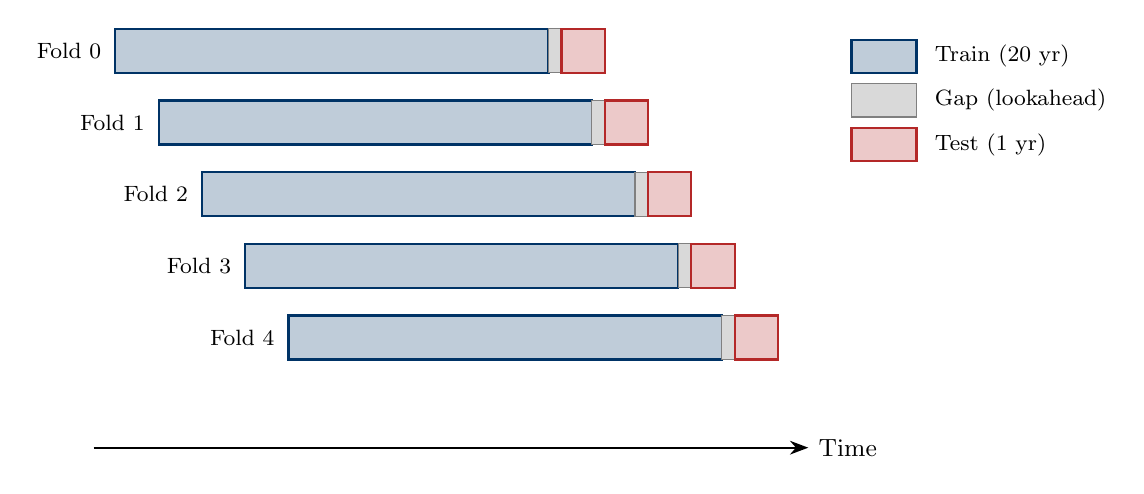
\begin{tikzpicture}[
  xscale=0.55, yscale=0.7,
  train/.style={fill=darkblue!25, draw=darkblue, thick},
  gap/.style={fill=gray!30, draw=gray},
  test/.style={fill=accent!25, draw=accent, thick},
  lbl/.style={font=\footnotesize}
]

\foreach \f/\ts/\te/\vs/\ve in {
  0/0/10/10.3/11.3,
  1/1/11/11.3/12.3,
  2/2/12/12.3/13.3,
  3/3/13/13.3/14.3,
  4/4/14/14.3/15.3
}{
  \draw[train] (\ts, -\f*1.3) rectangle (\te, -\f*1.3+0.8);
  \draw[gap]   (\te, -\f*1.3) rectangle (\vs, -\f*1.3+0.8);
  \draw[test]  (\vs, -\f*1.3) rectangle (\ve, -\f*1.3+0.8);
  \node[lbl, left] at (\ts-0.1, -\f*1.3+0.4) {Fold \f};
}

% Legend
\draw[train] (17, 0) rectangle (18.5, 0.6);
\node[font=\footnotesize, right] at (18.7, 0.3) {Train (20 yr)};
\draw[gap]   (17, -0.8) rectangle (18.5, -0.2);
\node[font=\footnotesize, right] at (18.7, -0.5) {Gap (lookahead)};
\draw[test]  (17, -1.6) rectangle (18.5, -1.0);
\node[font=\footnotesize, right] at (18.7, -1.3) {Test (1 yr)};

% Time arrow
\draw[-{Stealth}, thick] (-0.5, -6.8) -- (16, -6.8) node[right, font=\small] {Time};

\end{tikzpicture}
\end{frame}
%
%..................................................................
%
\begin{frame}{Time-Series Cross-Validation Design}

\begin{block}{\texttt{MultipleTimeSeriesCV} Parameters}
\centering\small
\begin{tabular}{lcl}
\toprule
\textbf{Parameter} & \textbf{Value} & \textbf{Meaning} \\
\midrule
\texttt{n\_splits} & 5 & Number of walk-forward folds \\
\texttt{train\_period\_length} & $20 \times 52 = 1040$ weeks & Training window \\
\texttt{test\_period\_length} & $1 \times 52 = 52$ weeks & Validation window \\
\texttt{lookahead} & 2 & Gap to prevent information leakage \\
\bottomrule
\end{tabular}
\end{block}

\end{frame}
%
%..................................................................
%
\begin{frame}[fragile]{Data Splitting: \texttt{get\_train\_valid\_data}}

\begin{lstlisting}
def get_train_valid_data(data, train_idx, val_idx):
    train, val = data.iloc[train_idx], data.iloc[val_idx]

    # Input 1: characteristics tensor (T, N, P)
    X1_train = train[characteristics].values.reshape(-1, n_tickers, n_characteristics)

    # Input 2: contemporaneous returns matrix (T, N)
    X2_train = train['returns'].unstack('ticker')

    # Target: forward returns (T, N)
    y_train  = train.returns_fwd.unstack('ticker')
    ...
    return X1_train, X2_train, y_train, X1_val, X2_val, y_val
\end{lstlisting}
\end{frame}
%
%..................................................................
%
\begin{frame}[fragile]{Data Splitting: \texttt{get\_train\_valid\_data}}

\begin{columns}[T]
\column{0.48\textwidth}
\begin{block}{Three Objects per Split}
\begin{itemize}
  \item \textbf{X1}: 3D tensor of characteristics\\$(T \times N \times 15)$ $\rightarrow$ beta network
  \item \textbf{X2}: return matrix\\$(T \times N)$ $\rightarrow$ factor network
  \item \textbf{y}: forward returns\\$(T \times N)$ $\rightarrow$ target
\end{itemize}
\end{block}

\column{0.48\textwidth}
\begin{block}{Key Assumption}
For each date, there are exactly \texttt{n\_tickers} rows in the panel.

\medskip

The \texttt{reshape(-1, n\_tickers, n\_characteristics)} relies on this regular structure to produce the 3D tensor.
\end{block}
\end{columns}

\end{frame}
%
%..................................................................
%
\begin{frame}[fragile]{Grid Search over Architecture Choices}

\begin{columns}[T]
\column{0.42\textwidth}
\begin{block}{Search Grid}
\begin{lstlisting}
factor_opts = [2, 3, 4, 5, 6]
unit_opts   = [8, 16, 32]

param_grid = list(
  product(unit_opts, factor_opts))
# -> 15 combinations
\end{lstlisting}
\end{block}

\column{0.55\textwidth}

\begin{block}{Training Protocol}
\begin{itemize}
  \item 250 epochs per fold
  \item Incremental fitting:\\
        \texttt{model.fit(epochs=e+1,\\ initial\_epoch=e)}
  \item Validation IC computed \textbf{after every epoch}
\end{itemize}
\end{block}

\begin{block}{Total Computation}
$$15 \text{ combos} \times 5 \text{ folds} \times 250 \text{ epochs} = 18{,}750 \text{ fit steps}$$
\end{block}

\end{columns}

\end{frame}
%
%..................................................................
%
\begin{frame}[fragile]{Grid Search over Architecture Choices}

\begin{exampleblock}{Evaluation Metric: Information Coefficient}
For each validation date $t$:
$$\mathrm{IC}_t = \mathrm{corr}_{\text{Spearman}}\bigl(\hat r_{i,t+1},\; r_{i,t+1}\bigr)$$
across all stocks $i$.

\medskip

Summarised as:
\begin{itemize}
  \item \textbf{IC mean}: average $\mathrm{IC}_t$ across dates
  \item \textbf{IC median}: robust central tendency
  \item \textbf{IC std}: stability of predictive skill
  \item \textbf{ICIR} $= \frac{\text{mean}(\mathrm{IC}_t)}{\text{std}(\mathrm{IC}_t)}$
\end{itemize}
\end{exampleblock}

\end{frame}
%
%..................................................................
%
\begin{frame}[fragile]{Inside the Training Loop}

\begin{lstlisting}
for units, n_factors in param_grid:
    model = make_model(hidden_units=units, n_factors=n_factors)
    for fold, (train_idx, val_idx) in enumerate(cv.split(data)):
        X1_train, X2_train, y_train, X1_val, X2_val, y_val = \
            get_train_valid_data(data, train_idx, val_idx)
        for epoch in range(250):
            model.fit([X1_train, X2_train], y_train, epochs=epoch+1,
                      initial_epoch=epoch, verbose=0, shuffle=True)
            # Predict and compute IC
            y_pred = model.predict([X1_val, X2_val]).reshape(-1)
            result = pd.DataFrame({'y_pred': y_pred, 'y_true': ...})
            r0 = spearmanr(result.y_true, result.y_pred)[0]    # pooled IC
            r1 = result.groupby('date').apply(                  # per-date IC
                lambda x: spearmanr(x.y_pred, x.y_true)[0])
            scores.append([units, n_factors, fold, epoch,
                           r0, r1.mean(), r1.std(), r1.median()])
\end{lstlisting}

\vspace{0.15cm}

Results are saved to HDF5 under keys like \texttt{"8/4"} (8 units, 4 factors) for later analysis.

\end{frame}
%__________________________________________________________________________
%
\subsection{Evaluation \& Model Selection}
%__________________________________________________________________________
%
\begin{frame}[fragile]{Aggregating Scores Across Folds}

\begin{lstlisting}
# Average IC metrics across folds for each (n_factors, units, epoch)
avg = (scores.groupby(['n_factors', 'units', 'epoch'])
       [['ic_mean', 'ic_daily_mean', 'ic_daily_median']]
       .mean().reset_index())

# For each hyperparameter pair, find the 5 best epochs
top = (avg.groupby(['n_factors', 'units'])
       .apply(lambda x: x.nlargest(5, 'ic_daily_median'))
       .reset_index(-1, drop=True))
\end{lstlisting}

\vspace{0.3cm}

\begin{block}{Why Average Across Folds?}
Each fold covers a different time period, so IC values fluctuate due to market regimes. Averaging across all 5 folds smooths out this temporal noise and gives a more reliable estimate of the model's \textbf{expected} predictive power for a given hyperparameter setting and training duration.
\end{block}

\end{frame}
%
%..................................................................
%
\begin{frame}{Cross-Validation Results --- Learning Curves}

\centering
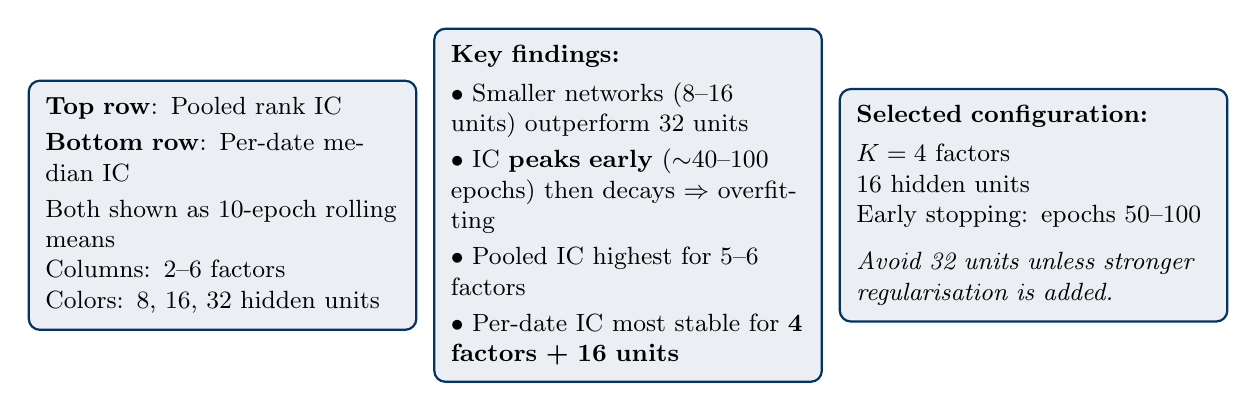
\begin{tikzpicture}[
  note/.style={draw=darkblue, thick, rounded corners, fill=darkblue!8,
               text width=4.5cm, align=left, font=\small, inner sep=6pt}
]
\node[note] (n1) at (0,0) {%
\textbf{Top row}: Pooled rank IC\\[2pt]
\textbf{Bottom row}: Per-date median IC\\[2pt]
Both shown as 10-epoch rolling means\\
Columns: 2--6 factors\\
Colors: 8, 16, 32 hidden units
};

\node[note, right=0.2cm of n1] (n2) {%
\textbf{Key findings:}\\[3pt]
$\bullet$ Smaller networks (8--16 units) outperform 32 units\\[2pt]
$\bullet$ IC \textbf{peaks early} ($\sim$40--100 epochs) then decays $\Rightarrow$ overfitting\\[2pt]
$\bullet$ Pooled IC highest for 5--6 factors\\[2pt]
$\bullet$ Per-date IC most stable for \textbf{4 factors + 16 units}
};

\node[note, right=0.2cm of n2] (n3) {%
\textbf{Selected configuration:}\\[3pt]
$K = 4$ factors\\
16 hidden units\\
Early stopping: epochs 50--100\\[6pt]
\textit{Avoid 32 units unless stronger regularisation is added.}
};
\end{tikzpicture}

\end{frame}
%
%..................................................................
%
\begin{frame}[fragile]{Ensemble Predictions over Epoch Range}

Instead of picking a single ``best epoch,'' we \textbf{average predictions} across epochs 50--100:

\begin{lstlisting}
n_factors, units, batch_size = 4, 16, 16
first_epoch, last_epoch = 50, 100

for epoch in tqdm(range(first_epoch, last_epoch)):
    epoch_preds = []
    for fold, (train_idx, val_idx) in enumerate(cv.split(data)):
        X1_train, X2_train, y_train, X1_val, X2_val, y_val = \
            get_train_valid_data(data, train_idx, val_idx)
        model = make_model(n_factors=n_factors, hidden_units=units)
        model.fit([X1_train, X2_train], y_train, epochs=epoch, verbose=0)
        epoch_preds.append(pd.Series(
            model.predict([X1_val, X2_val]).reshape(-1),
            index=y_val.stack().index).to_frame(epoch))
    predictions.append(pd.concat(epoch_preds))

predictions_combined = pd.concat(predictions, axis=1).sort_index()
\end{lstlisting}
\end{frame}
%
%..................................................................
%
\begin{frame}[fragile]{Ensemble Predictions over Epoch Range}

The result is a DataFrame with one column per epoch (50--99) and rows indexed by \texttt{(date, ticker)}. Averaging across columns yields a \textbf{smoothed ensemble forecast}.

\end{frame}
%
%..................................................................
%
\begin{frame}{Why Epoch Averaging?}

\begin{columns}[T]
\column{0.48\textwidth}
\begin{block}{The Problem}
\begin{itemize}
  \item Neural network predictions vary with the number of training epochs
  \item A single epoch checkpoint is \textbf{noisy}: small changes in stopping time produce different forecasts
  \item The optimal epoch differs across folds and market regimes
\end{itemize}
\end{block}

\column{0.48\textwidth}
\begin{block}{The Solution}
\begin{itemize}
  \item Train for every epoch in $[50, 100)$
  \item Collect out-of-sample predictions at each checkpoint
  \item \textbf{Average} across epochs to smooth prediction noise
  %\item Analogous to \textbf{snapshot ensembling} in deep learning
\end{itemize}
\end{block}
\end{columns}

%\vspace{0.4cm}

\begin{alertblock}{Important Detail}
For each epoch, the model is trained \textbf{from scratch} (fresh random initialisation).
This means each epoch column represents an independent model trained for exactly that many epochs --- not a continuation of the same training run.
\end{alertblock}

\end{frame}
%__________________________________________________________________________
%
\subsection{Section Summary}
%__________________________________________________________________________
%
\begin{frame}{Summary \& Key Takeaways}

\begin{columns}[T]
\column{0.48\textwidth}
\small
\begin{block}{What We Built}
\begin{enumerate}
  \item A \textbf{conditional autoencoder} that learns latent factors from returns, with loadings conditioned on firm characteristics
  \item A \textbf{walk-forward CV} pipeline respecting temporal ordering
  \item An \textbf{ensemble prediction} scheme averaging over epoch checkpoints
\end{enumerate}
\end{block}
\vspace{-.2cm}
\begin{block}{Selected Hyperparameters}
\footnotesize
\centering
\begin{tabular}{lc}
\toprule
Latent factors $K$ & 4 \\
Hidden units & 16 \\
Epoch range & 50--100 \\
Batch size & 16 \\
\bottomrule
\end{tabular}
\end{block}

\column{0.48\textwidth}
\begin{block}{Lessons for Students}
\begin{itemize}
  \item \textbf{Structure matters}: the dot-product output enforces economic interpretability ($r = \beta' f$)
  \item \textbf{Less is more}: smaller networks generalise better on noisy financial data
  %\item \textbf{Early stopping is critical}: IC degrades with overtraining
  \item \textbf{Rank normalisation} tames outliers without losing information
  \item \textbf{IC and ICIR} are the standard metrics for evaluating cross-sectional return predictors
\end{itemize}
\end{block}
\end{columns}

\vspace{0.3cm}
\centering
\Large\textbf{Thank you!}

\end{frame}
%__________________________________________________________________________
%
\section{Performance Evaluation of Alpha Factors with Alphalens}
%__________________________________________________________________________
%
\begin{frame}{Alphalens Evaluation Pipeline}

\begin{columns}[T]
\column{0.48\textwidth}
\begin{block}{Setup}
\begin{itemize}
  \item Epoch-averaged predictions $\rightarrow$ single factor score per (date, ticker)
  \item Aligned with weekly trade prices (Friday, UTC)
  \item Holding periods: 5D, 10D, 21D
  \item 5 quintiles ($Q=5$)
\end{itemize}
\end{block}

\begin{block}{Alphalens Key Function}
\texttt{get\_clean\_factor\_and\_forward\_returns}\\
merges factor scores with realised forward returns and assigns quantiles. $\sim$18.5\% observations dropped (missing fwd returns).
\end{block}

\column{0.48\textwidth}
\begin{block}{Diagnostics Produced}
\begin{enumerate}
  \item \textbf{Quantile returns}: bar charts, cumulative lines, violin plots
  \item \textbf{Alpha \& Beta}: factor regressed on market return
  \item \textbf{Information Coefficient}: distribution, time series, monthly heatmap
  \item \textbf{Turnover}: quantile composition stability, rank autocorrelation
  \item \textbf{Summary \& full tear sheets}
\end{enumerate}
\end{block}
\end{columns}

\end{frame}
%
%..................................................................
%
\begin{frame}{Quantile Returns: Monotonic Cross-Sectional Ordering}

\begin{columns}[T]
\column{0.48\textwidth}
\begin{block}{Cumulative Returns by Quantile}
\begin{itemize}
  \item \textbf{5D horizon}: clear monotonic spread; Q5 outperforms, Q1 underperforms
  \item \textbf{10D}: ordering persists, spread slightly narrows
  \item \textbf{21D}: structure still visible but weaker $\Rightarrow$ signal is primarily \textbf{short-term}
\end{itemize}
\end{block}
\vspace{-.3cm}
\begin{block}{Long--Short Spread (Q5 $-$ Q1)}
\centering\small
\begin{tabular}{lc}
\toprule
Horizon & Mean Spread (bps) \\
\midrule
5D & 31.4 \\
10D & 16.8 \\
21D & 17.8 \\
\bottomrule
\end{tabular}
\end{block}

\column{0.48\textwidth}
\begin{block}{Alpha \& Beta vs.\ Market}
\centering\small
\begin{tabular}{lccc}
\toprule
& 5D & 10D & 21D \\
\midrule
Ann.\ Alpha & 3.05\% & 0.70\% & 3.44\% \\
Beta & 0.062 & 0.054 & 0.009 \\
\bottomrule
\end{tabular}

\medskip
\raggedright
Near-zero betas confirm the factor is \textbf{orthogonal to the market}: it captures \textbf{idiosyncratic}, firm-specific predictive content.
\end{block}
\end{columns}
\end{frame}
%
%..................................................................
%
\begin{frame}{Quantile Returns: Monotonic Cross-Sectional Ordering}
\vspace{0.5cm}
\begin{exampleblock}{Economic Interpretation}
The CAE compresses 15 characteristics into a latent score that ranks stocks by expected return. The ranking is stable, monotonic, and market-independent.
\end{exampleblock}
\end{frame}
%
%..................................................................
%
\begin{frame}{Information Coefficient Analysis}

\begin{columns}[T]
\column{0.48\textwidth}
\begin{block}{IC Summary Statistics}
\centering\small
\begin{tabular}{lccc}
\toprule
& 5D & 10D & 21D \\
\midrule
IC Mean & 0.008 & 0.004 & 0.009 \\
IC Std & 0.053 & 0.047 & 0.041 \\
Risk-Adj.\ IC & 0.146 & 0.095 & 0.229 \\
$t$-stat & 2.27 & 1.47 & 3.54 \\
$p$-value & 0.024 & 0.142 & 0.000 \\
\bottomrule
\end{tabular}
\end{block}

\vspace{-0.3cm}

\begin{block}{Key Observations}
\begin{itemize}
  \item IC positive at \textbf{all horizons}
  \item Statistically significant at 5D ($p{=}0.024$) and 21D ($p{<}0.001$)
  %\item IC distributions are \textbf{near-Gaussian} (Q-Q plots confirm)
  %\item IC std \textbf{decreases} with horizon $\Rightarrow$ increased signal stability
\end{itemize}
\end{block}

\column{0.48\textwidth}
\begin{block}{Temporal Dynamics}
\begin{itemize}
  \item Rolling IC oscillates around zero with recurrent \textbf{positive phases}
  \item Sustained strength 2016--2017; brief weakness during late-2018 volatility
  \item Monthly IC heatmaps: \textbf{predominantly blue} (positive), especially at 21D
  \item No persistent structural breakdowns detected
\end{itemize}
\end{block}
\end{columns}
\end{frame}
%
%..................................................................
%
\begin{frame}{Information Coefficient Analysis}

\begin{alertblock}{Interpretation}
The CAE factor provides a \textbf{statistically significant, temporally stable} predictive signal. Magnitudes ($\text{IC} \approx 0.01$) are typical for equity factors and sufficient for economically meaningful strategies when applied with high breadth.
\end{alertblock}

\end{frame}
%
%..................................................................
%
\begin{frame}{Turnover \& Signal Persistence}

\begin{columns}[T]
\column{0.48\textwidth}
\begin{block}{Quantile Turnover}
\centering\small
\begin{tabular}{lccc}
\toprule
Quantile & 5D & 10D & 21D \\
\midrule
Q1 & 0.496 & 0.572 & 0.644 \\
Q3 & 0.655 & 0.697 & 0.734 \\
Q5 & 0.490 & 0.568 & 0.640 \\
\bottomrule
\end{tabular}

\medskip
\raggedright
Turnover in the 0.49--0.75 range. Extreme quintiles (Q1, Q5) are the \textbf{most stable}, suggesting persistent rankings at the tails.
\end{block}

\column{0.48\textwidth}
\begin{block}{Factor Rank Autocorrelation}
\centering\small
\begin{tabular}{lc}
\toprule
Horizon & Mean Autocorr. \\
\midrule
5D & 0.511 \\
10D & 0.399 \\
21D & 0.286 \\
\bottomrule
\end{tabular}

\medskip
\raggedright
Smooth decay from 0.51 to 0.29: the signal persists for \textbf{1--3 weeks} before dissipating. This is consistent with short-to-medium-term equity factors.
\end{block}
\end{columns}
\end{frame}
%
%..................................................................
%
\begin{frame}{Turnover \& Signal Persistence}

\begin{exampleblock}{Balance Between Adaptability and Persistence}
The model updates frequently enough to incorporate new information while maintaining stable rankings, avoiding excessive transaction costs. Turnover spikes coincide with market volatility, not model instability.
\end{exampleblock}

\end{frame}
%
%..................................................................
%
\begin{frame}{Summary of Findings}

\begin{block}{What the Results Suggest}
The conditional autoencoder:
\begin{enumerate}
  \item \textbf{Orders the cross-section coherently}: monotonic Q1--Q5 return spreads at all horizons
  \item \textbf{Delivers market-orthogonal alpha}: annualised $\alpha \approx 3\%$, $\beta \approx 0$ vs.\ the market
  \item \textbf{Produces statistically significant ICs}: $t$-stat $> 2$ at 5D and 21D
  \item \textbf{Remains temporally stable}: no structural breakdowns across 2015--2019
  \item \textbf{Balances adaptability and persistence}: smooth turnover, rank autocorrelation decays naturally
\end{enumerate}
\end{block}

\vspace{0.2cm}

\begin{block}{Conceptual Contribution}
The CAE bridges \textbf{economic structure} (conditional factor model, no-arbitrage) with \textbf{deep learning flexibility} (nonlinear loadings, data-driven factors). It demonstrates that interpretability and complexity are \textbf{complementary}, not opposing.
\end{block}

\end{frame}
%__________________________________________________________________________
%
%\appendix
%__________________________________________________________________________
%
\section{Appendix A\\ Keras}
%__________________________________________________________________________
%
\begin{frame}{What Is Keras? --- The 5-Step Workflow}

\begin{columns}[T]
\column{0.50\textwidth}
\small
\textbf{Keras} is the high-level API of TensorFlow for building and training neural networks. Accessible as \texttt{tensorflow.keras}.

\vspace{0.15cm}

\begin{block}{\small Key Characteristics}
\footnotesize
\begin{itemize}\setlength\itemsep{1pt}
  \item \textbf{Modular}: models = layers snapped together
  \item \textbf{Two APIs}: Sequential (simple) and Functional (complex)
  \item \textbf{Extensible}: custom layers, losses, callbacks
  \item Runs on CPU, GPU, and TPU
\end{itemize}
\end{block}

\column{0.46\textwidth}
\centering
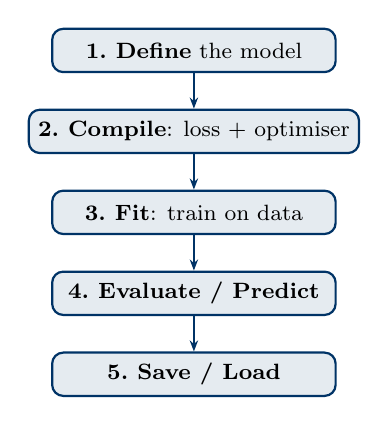
\begin{tikzpicture}[
  node distance=0.45cm,
  box/.style={draw=darkblue, thick, rounded corners, fill=darkblue!10,
              minimum width=3.6cm, minimum height=0.55cm, align=center,
              font=\footnotesize},
  arr/.style={-{Stealth[length=4pt]}, thick, darkblue}
]
\node[box] (d) {\textbf{1.\ Define} the model};
\node[box, below=of d] (c) {\textbf{2.\ Compile}: loss + optimiser};
\node[box, below=of c] (f) {\textbf{3.\ Fit}: train on data};
\node[box, below=of f] (e) {\textbf{4.\ Evaluate / Predict}};
\node[box, below=of e] (s) {\textbf{5.\ Save / Load}};
\draw[arr] (d)--(c); \draw[arr] (c)--(f);
\draw[arr] (f)--(e); \draw[arr] (e)--(s);
\end{tikzpicture}
\end{columns}

\end{frame}
%
%..................................................................
%
\begin{frame}[fragile]{Sequential vs.\ Functional API}

\begin{columns}[T]
\column{0.48\textwidth}
\begin{block}{\small Sequential --- Single Chain of Layers}
\begin{lstlisting}
from tensorflow.keras.models import Sequential
from tensorflow.keras.layers import Dense, Dropout

model = Sequential([
  Dense(64, activation='relu',
        input_shape=(15,)),
  Dropout(0.2),
  Dense(32, activation='relu'),
  Dense(1)          # regression output
])
\end{lstlisting}
\footnotesize One input, one output, no branching.
\end{block}

\column{0.48\textwidth}
\begin{block}{\small Functional --- Multi-Input / Branching}
\begin{lstlisting}
from tensorflow.keras.layers import (
    Input, Dense, BatchNormalization, Dot)
from tensorflow.keras.models import Model

inp_chars = Input((N, P), name='chars')
inp_ret   = Input((N,),   name='returns')
# Branch 1
x = Dense(8, activation='relu')(inp_chars)
x = BatchNormalization()(x)
betas = Dense(K)(x)
# Branch 2
factors = Dense(K)(inp_ret)
# Merge
out = Dot(axes=(2,1))([betas, factors])

model = Model([inp_chars, inp_ret], out)
\end{lstlisting}
\end{block}
\end{columns}

%\vspace{0.15cm}
%\footnotesize\textbf{Rule of thumb}: start with Sequential; switch to Functional when you need multiple inputs/outputs or shared layers (e.g.\ the conditional autoencoder).

\end{frame}
%
%..................................................................
%
\begin{frame}{Core Layers \& Activations}

\begin{columns}[T]
\column{0.52\textwidth}
\begin{block}{\small Essential Layers}
\footnotesize
\renewcommand{\arraystretch}{1.15}
\begin{tabular}{@{}lp{4.5cm}@{}}
\toprule
\textbf{Layer} & \textbf{Purpose} \\
\midrule
\texttt{Dense(n, act)} & Fully connected: $g(Wx{+}b)$ \\
\texttt{Dropout(rate)} & Randomly zeros units (regularisation) \\
\texttt{BatchNorm()} & Normalise activations to $\mu{=}0,\sigma{=}1$ \\
\texttt{Input(shape)} & Declares entry point (Functional API) \\
\texttt{Dot(axes)} & Dot product of two tensors \\
\texttt{Flatten()} & Collapse dims to 1D vector \\
\bottomrule
\end{tabular}
\end{block}

\column{0.45\textwidth}
\begin{block}{\small Activation Functions}
\footnotesize
\renewcommand{\arraystretch}{1.15}
\begin{tabular}{@{}llp{2cm}@{}}
\toprule
\textbf{Name} & \textbf{Formula} & \textbf{Use} \\
\midrule
\texttt{relu} & $\max(0,x)$ & Hidden layers \\
\texttt{sigmoid} & $\frac{1}{1+e^{-x}}$ & Binary output \\
\texttt{softmax} & $\frac{e^{x_i}}{\sum e^{x_j}}$ & Multi-class \\
\texttt{linear} & $x$ & Regression \\
\bottomrule
\end{tabular}
\end{block}

\vspace{0.15cm}

\begin{exampleblock}{\small Practical Rule}
\footnotesize
\texttt{relu} in hidden layers.\\ Output activation depends on the task: \texttt{linear} for regression, \texttt{sigmoid}/\texttt{softmax} for classification.
\end{exampleblock}
\end{columns}

\end{frame}
%
%..................................................................
%
\begin{frame}[fragile]{Compile \& Fit}

\begin{columns}[T]
\column{0.48\textwidth}
\begin{block}{\small Step 2: Compile}
\begin{lstlisting}
model.compile(
  loss='mse',          # what to minimise
  optimizer='adam',     # how to update weights
  metrics=['mae'])     # what to monitor
\end{lstlisting}
\end{block}

\vspace{0.1cm}

\footnotesize
\renewcommand{\arraystretch}{1.1}
\begin{tabular}{@{}ll@{}}
\toprule
\textbf{Task} & \textbf{Loss} \\
\midrule
Regression & \texttt{mse}, \texttt{mae} \\
Binary classif. & \texttt{binary\_crossentropy} \\
Multi-class & \texttt{categorical\_crossentropy} \\
\bottomrule
\end{tabular}

\medskip

\textbf{Adam} is the default go-to optimiser: adaptive learning rate + momentum.

\column{0.48\textwidth}
\begin{block}{\small Step 3: Fit (Train)}
\begin{lstlisting}
history = model.fit(
  X_train, y_train,
  epochs=100,          # full passes over data
  batch_size=32,       # samples per update
  validation_data=(X_val, y_val),
  shuffle=True,
  verbose=1)
\end{lstlisting}
\end{block}

\vspace{0.1cm}

\footnotesize
\texttt{history.history} stores train/val loss per epoch.

\medskip

\textbf{Diagnosing overfitting via learning curves:}\\
Train loss $\downarrow$, val loss $\uparrow$ $\Rightarrow$ overfitting\\
Both $\downarrow$ $\Rightarrow$ keep training\\
Both flat $\Rightarrow$ converged

\end{columns}

\end{frame}
%
%..................................................................
%
\begin{frame}[fragile]{Evaluate, Predict, Save}

\begin{lstlisting}
# Step 4: Evaluate on held-out test data (returns loss + metrics)
test_loss, test_mae = model.evaluate(X_test, y_test, verbose=0)

# Step 4: Generate predictions (forward pass only, no gradient)
y_pred = model.predict(X_new)

# Step 5: Save entire model (architecture + weights + optimiser)
model.save('my_model.keras')

# Step 5: Reload later
from tensorflow.keras.models import load_model
model = load_model('my_model.keras')
\end{lstlisting}

\vspace{0.2cm}

\begin{columns}[T]
\column{0.48\textwidth}
\begin{block}{\small \texttt{model.summary()}}
\footnotesize
Call immediately after building to verify layer shapes and parameter counts. Catches dimensionality errors early.
\end{block}

\column{0.48\textwidth}
\begin{block}{\small Weights-Only Save}
\footnotesize
\texttt{model.save\_weights('w.h5')} saves only the trained parameters (lighter). Requires re-building the architecture before loading.
\end{block}
\end{columns}

\end{frame}
%
%..................................................................
%
\begin{frame}[fragile]{Controlling Overfitting}

\begin{columns}[T]
\column{0.48\textwidth}
\begin{block}{\small Dropout}
\begin{lstlisting}
Dense(64, activation='relu'),
Dropout(0.3),  # drop 30% of units
Dense(32, activation='relu'),
\end{lstlisting}
\footnotesize
Randomly disables neurons during training. Off at prediction time.
\end{block}

\vspace{0.1cm}

\begin{block}{\small $L_2$ Weight Regularisation}
\begin{lstlisting}
from tensorflow.keras.regularizers import l2
Dense(64, activation='relu',
      kernel_regularizer=l2(1e-4))
\end{lstlisting}
\footnotesize
Adds $\lambda\|W\|_2^2$ to the loss, shrinking weights.
\end{block}

\column{0.48\textwidth}
\begin{block}{\small Batch Normalisation}
\begin{lstlisting}
Dense(64, activation='relu'),
BatchNormalization(),
\end{lstlisting}
\footnotesize
Normalises activations per mini-batch. Stabilises training and acts as mild regulariser.
\end{block}

\vspace{0.1cm}

\begin{block}{\small Early Stopping}
\begin{lstlisting}
from tensorflow.keras.callbacks \
    import EarlyStopping
es = EarlyStopping(monitor='val_loss',
       patience=10,
       restore_best_weights=True)
model.fit(..., callbacks=[es])
\end{lstlisting}
\footnotesize
Stops training when val loss stops improving.
\end{block}
\end{columns}

\end{frame}
%
%..................................................................
%
\begin{frame}[fragile]{Callbacks \& Multi-Input Models}

\begin{columns}[T]
\column{0.48\textwidth}
\begin{block}{\small Useful Callbacks}
\footnotesize
\renewcommand{\arraystretch}{1.15}
\begin{tabular}{@{}lp{3.5cm}@{}}
\toprule
\textbf{Callback} & \textbf{What It Does} \\
\midrule
\texttt{EarlyStopping} & Stop when metric plateaus \\
\texttt{ModelCheckpoint} & Save best weights \\
\texttt{ReduceLROnPlateau} & Lower LR on plateau \\
\texttt{TensorBoard} & Interactive log viewer \\
\texttt{CSVLogger} & Metrics to CSV file \\
\bottomrule
\end{tabular}
\end{block}

\vspace{-0.1cm}

\begin{lstlisting}
callbacks = [
  EarlyStopping(monitor='val_loss',
    patience=10,
    restore_best_weights=True),
  ModelCheckpoint('best.keras',
    save_best_only=True)]
model.fit(..., callbacks=callbacks)
\end{lstlisting}

\column{0.48\textwidth}
\begin{block}{\small Multi-Input Pattern}
\begin{lstlisting}
inp_a = Input((10,), name='numeric')
inp_b = Input((50,), name='text')
a = Dense(32, activation='relu')(inp_a)
b = Dense(64, activation='relu')(inp_b)
merged = Concatenate()([a, b])
out = Dense(1)(merged)

model = Model([inp_a, inp_b], out)
\end{lstlisting}
\footnotesize
Use the Functional API whenever you need multiple inputs, multiple outputs, or shared layers.

\medskip

The \textbf{conditional autoencoder} uses exactly this pattern: two inputs (\texttt{characteristics}, \texttt{returns}) merged via \texttt{Dot}.
\end{block}
\end{columns}

\end{frame}
%
%..................................................................
%
\begin{frame}{Summary --- What to Remember}

\begin{columns}[T]
\column{0.48\textwidth}
\begin{block}{\small The 5-Step Mental Model}
\footnotesize
\begin{enumerate}\setlength\itemsep{2pt}
  \item \textbf{Define}: stack layers (Sequential or Functional)
  \item \textbf{Compile}: pick loss + optimiser
  \item \textbf{Fit}: train, monitor validation
  \item \textbf{Predict}: forward pass only
  \item \textbf{Save}: persist for later use
\end{enumerate}
\end{block}

\vspace{0.15cm}

\begin{block}{\small Most-Used Layers}
\footnotesize
\texttt{Input} $\cdot$ \texttt{Dense} $\cdot$ \texttt{Dropout} $\cdot$ \texttt{BatchNormalization} $\cdot$ \texttt{Dot} $\cdot$ \texttt{Concatenate} $\cdot$ \texttt{Flatten}
\end{block}

\column{0.48\textwidth}
\begin{block}{\small Practical Tips}
\footnotesize
\begin{itemize}\setlength\itemsep{2pt}
  \item \texttt{relu} hidden layers, \texttt{linear} regression output
  \item Start with \texttt{adam}, default LR ($10^{-3}$)
  \item Always use a \textbf{validation set}
  \item Add \texttt{EarlyStopping} to save compute
  \item Call \texttt{model.summary()} to check shapes
  \item Plot learning curves --- they tell you everything
\end{itemize}
\end{block}

\vspace{0.15cm}

\begin{exampleblock}{\small Golden Rule}
\footnotesize
Start simple, inspect \texttt{summary()}, plot learning curves, then iterate. Add complexity only when validation loss demands it.
\end{exampleblock}
\end{columns}

\end{frame}
%__________________________________________________________________________
%
\section{Appendix B\\ The Alphalens Library}
%__________________________________________________________________________
%
\begin{frame}{Appendix --- Alphalens: Overview}

\begin{block}{What Is Alphalens?}
\textbf{Alphalens} is an open-source Python library originally developed by \textbf{Quantopian} for the \textbf{performance analysis of predictive alpha factors}. It is designed to answer a single question: \emph{does a given signal actually predict future returns?}
\end{block}
\vspace{-.5cm}
\begin{columns}[T]
\column{0.48\textwidth}
\begin{block}{Core Capabilities}
\begin{itemize}
  \item Correlation of signals with subsequent returns
  \item Profitability of equal- or factor-weighted quantile portfolios
  \item Factor turnover and implied trading costs
  \item Factor performance during specific events
  \item Sector-level breakdowns of all metrics
\end{itemize}
\end{block}

\column{0.48\textwidth}
\begin{block}{Ecosystem Integration}
\begin{itemize}
  \item \textbf{Zipline}: event-driven backtesting engine that produces the signals Alphalens analyses
  \item \textbf{Pyfolio}: portfolio-level risk and return analytics (Sharpe, drawdowns, etc.)
  \item Together: \textbf{signal $\rightarrow$ backtest $\rightarrow$ portfolio analysis}
\end{itemize}
\end{block}
\end{columns}

\end{frame}
%
%..................................................................
%
\begin{frame}{Appendix --- Alphalens: Module Structure}
\footnotesize
Alphalens is organised into four main modules:

\vspace{0.3cm}

\renewcommand{\arraystretch}{1.35}
\centering
\begin{tabular}{@{}lp{10cm}@{}}
\toprule
\textbf{Module} & \textbf{Purpose} \\
\midrule
\texttt{alphalens.utils} &
  Data preparation. The key function \texttt{get\_clean\_factor\_and\_forward\_returns} merges factor signals with forward returns and assigns quantiles. Also handles date alignment, NaN cleaning, and sector mapping. \\
\texttt{alphalens.performance} &
  Computational engine. Functions to compute mean returns by quantile, the Information Coefficient (IC), factor-weighted returns, cumulative returns, and turnover metrics. \\
\texttt{alphalens.plotting} &
  Visualisation layer. One plotting function per analysis type: bar charts, line plots, violin plots, heatmaps, and time-series IC charts. \\
\texttt{alphalens.tears} &
  Tear sheets. High-level convenience functions that combine multiple \texttt{performance} computations and \texttt{plotting} calls into comprehensive one-call reports. \\
\bottomrule
\end{tabular}

\end{frame}
%
%..................................................................
%
\begin{frame}[fragile]{Appendix --- Alphalens: Key Functions Reference}

\small

\textbf{Data Preparation} (\texttt{utils})
\begin{lstlisting}
alphalens.utils.get_clean_factor_and_forward_returns(
    factor,              # Series with MultiIndex (date, asset)
    prices,              # DataFrame: dates x assets
    periods=(1,5,10),    # holding periods in trading days
    quantiles=5,         # number of signal bins
    bins=None,           # alternative: custom bin edges
    filter_zscore=20,    # drop extreme forward returns
    groupby=None)        # optional sector grouping
\end{lstlisting}

\textbf{Performance Computations} (\texttt{performance})
\begin{lstlisting}
mean_return_by_quantile(factor_data, by_date=False, by_group=False)
factor_information_coefficient(factor_data, group_adjust=False, by_group=False)
factor_returns(factor_data, long_short=True, group_neutral=False)
average_cumulative_return_by_quantile(factor_data, prices, periods_before, ...)
quantile_turnover(quantile_factor, quantile, period=1)
factor_rank_autocorrelation(factor_data, period=1)
\end{lstlisting}

\end{frame}
%
%..................................................................
%
\begin{frame}[fragile]{Appendix --- Alphalens: Plotting \& Tear Sheets}

\small

\textbf{Plotting Functions} (\texttt{plotting})
\begin{lstlisting}
plot_quantile_returns_bar(mean_return_by_q)
plot_cumulative_returns_by_quantile(mean_return_by_q_daily, period)
plot_quantile_returns_violin(return_by_q)
plot_ic_ts(ic, ax=None)                       # IC time series
plot_ic_hist(ic, ax=None)                      # IC histogram
plot_ic_qq(ic, ax=None)                        # IC Q-Q plot
plot_ic_heatmap(ic, ax=None)                   # monthly IC heatmap
plot_turnover_table(autocorrelation_data, quantile_turnover)
plot_top_bottom_quantile_turnover(quantile_turnover, period)
plot_factor_rank_auto_correlation(factor_autocorrelation)
\end{lstlisting}

\vspace{0.2cm}

\textbf{Tear Sheet Functions} (\texttt{tears})
\begin{lstlisting}
create_summary_tear_sheet(factor_data)             # all-in-one report
create_returns_tear_sheet(factor_data)             # returns analysis only
create_information_tear_sheet(factor_data)          # IC analysis only
create_turnover_tear_sheet(factor_data)             # turnover analysis only
create_event_returns_tear_sheet(factor_data, prices, ...)  # event study
create_full_tear_sheet(factor_data)                # everything combined
\end{lstlisting}

\end{frame}
%
%===================================================================================================
%
\end{document}
